\clearpage
\section{Praktischer Selbstversuch}
\label{sec:practice}

Um die Schlussfolgerungen aus dem Forschungsteil weiter zu untersuchen, wurde entschieden, die Vor- und Nachteile der Lerntypen in einem praktischen Selbstversuch zu betrachten.
Es soll hierbei speziell untersucht werden, welche Schwierigkeiten erwartet werden, und welche tatsächlich bei der Bearbeitung auftreten.
Hierzu werden die einzelnen Lerndimensionen der Autorin untersucht. Anschließend wird ein einfacher Algorithmus in einer funktionalen Programmiersprache umgesetzt. Es wurde sich für Haskell entschieden, da es die meistverwendete funktionale Programmiersprache in Einsteigerkursen im Bereich Informatik ist (siehe \nameref{sec:curriculares}).
Zur Vorbereitung wurde der Kurs CIS 194 \cite{cis194} der University of Pennsylvania genutzt, der in der offiziellen Haskell-Dokumentation empfohlen wird \cite{haskelldoc}.
Als Problem wurde "Türme von Hanoi" gewählt. Weitere Erläuterungen zu der Art des Problems folgen in Abschnitt \nameref{sec:problemdesc}.

\subsection{Lerntypenanalyse}
Um den Selbstversuch mit den Vor- und Nachteilen der Lerntypen zu verbinden, musste zunächst eine eigene Lerntypenanalyse durchgeführt werden.
Hierzu wurde der "Index of Learning Styles Questionnaire" verwendet \cite{ils_questionnaire}, ein Online-Tool, welches insgesamt 44 Fragen stellt und dann auf Basis der Antworten die Lerntypen eines Individuums einschätzen kann. Die Lerntypen werden als Gegensatzpaare auf einer Skala gezeigt, die darstellen soll, wie ausgeprägt der Hang zu einem Aspekt ist. Ein Wert von 1 bis 3 entspricht einer ausgewogenen Balance beider Aspekte der Dimension mit leichten Präferenzen, 5 bis 7 entspricht einem mäßigen Hang zu einem Aspekt und 9 bis 11 entspricht einer starken Präferenz für einen der Lernstile.
Die Verlässlichkeit dieses Fragebogens wurde sowohl von den ursprünglichen Verfassenden des Lernmodells \cite{felder2005} als auch von anderen Quellen \cite{zywno} geprüft und bestätigt.

Die Fragen des ILS Fragebogens wurden in einer zufälligen Reihenfolge beantwortet, um zu vermeiden, dass bereits vorab klar ist, welche Frage welcher Typendimension zugeordnet ist. Dies ist möglich, da der Test so aufgebaut ist, dass jeweils ein Frageblock von 4 Fragen jede Dimension behandelt. Die erste Frage beispielsweise fließt in die Bewertung der aktiv/reflexiven Dimension ein, ebenso wie die fünfte und neunte Frage.

\subsubsection{Ergebnisse der persönlichen Evaluierung}
Der Fragebogen wurde Online auf der offiziellen Seite der University of Pennsylvania bearbeitet. Die Ergebnisse des Fragebogens lauten wie folgt.

\begin{figure}[H]
    \centering
    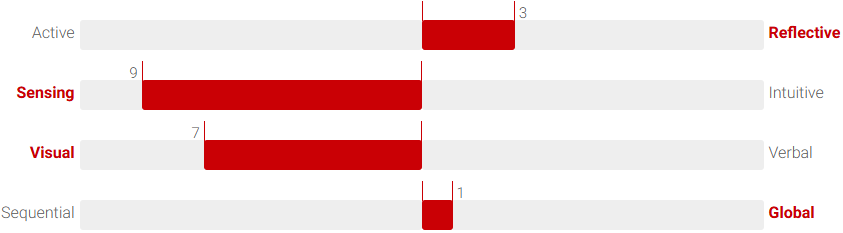
\includegraphics[width=1\linewidth]{Figures/Section_4/ILS_result}
    \caption{Ergebnisse des ILS Fragebogens}
\end{figure}

Die Autorin zeigt demnach folgende Ausprägungen in den Dimensionen.

\begin{itemize}
    \item Ein ausgewogenes Verhältnis der aktiven/reflexiven Dimension, möglicherweise eine leichte Präferenz für den aktiven Typ
    \item Eine starke Präferenz für den sensorischen Typ
    \item Eine mäßige Präferenz für den visuellen Typ
    \item Ein ausgewogenes Verhältnis der sequenziellen/globalen Dimension, möglicherweise eine leichte Präferenz für den globalen Typ
\end{itemize}

Die individuellen Ausprägungen der Lerntypen werden im praktischen Versuch hinsichtlich des Erlernens und Anwendens der CT Aspekte und der verschiedenen Paradigmen untersucht.
Die Ausprägungen sollten sich demnach wie folgt auswirken.

\begin{itemize}
    \item Ein leichter Nachteil beim Debugging in funktionaler Programmierung (FP), und beim Erlernen von Programmieren in Einzelarbeit, allerdings auch ein schnelleres Ausprobieren von Ansätzen
    \item Ein Nachteil beim Anwenden von algorithmischem Denken und der Erkennung der Zusammenhänge zwischen FP und mathematischen Funktionen, sowie beim innovativen Arbeiten mit einem limitierten Toolset. Demnach ebenfalls ein Nachteil bei der Findung von rekursiven Lösungsansätzen
    \item Ein möglicher mäßiger Vorteil bei der Dekomposition aus der Perspektive eines visuellen Lerntypen, allerdings ein Nachteil bei der Abstraktion aufgrund einer eher sensorischen Ausprägung
    \item Kein besonderer zusätzlicher Vorteil bei der Dekomposition aus der Perspektive eines sequenziellen Lerntyps, sowie der generellen Anwendung von FP in einer sequenziellen Lösungsstrategie
\end{itemize}

\subsection{Problembeschreibung}\label{sec:problemdesc}
Um die aufgestellten Thesen zu prüfen, wurde entschieden, eine Programmieraufgabe in einem praktischen Teil zu lösen und alle Erfahrungen, Schwierigkeiten und Probleme in einer Art "Development Diary" zu dokumentieren.
Als Problem für den praktischen Versuch wurden die "Türme von Hanoi" gewählt. Diese Entscheidung wurde getroffen, da die Aufgabe in einem Anfängerkurs mit eigener Aufgabenstellung vertreten war \cite{cis194}, sowie alle Aspekte des CT abdeckt (siehe \nameref{sec:choice_prac}). Das Problem erfordert zudem die Anwendung von Rekursion, was in der FP einen besonderen Stellenwert hat.
Die Aufgabenstellung des Kurses CIS 194 bietet einen Ansatz in Form einer vorgegebenen Funktionsdefinition, sowie zwei vordefinierten Datentypen. Aufgrund dessen, dass auch der Aspekt der Abstraktion und Dekomposition betrachtet werden sollte, wurde die Aufgabenstellung des Kurses CIS 194 nicht verwendet. Stattdessen wurde von Grund auf selbst eine Lösung gefunden.

In dem Problem geht es um drei Holzstäbe, auf denen unterschiedlich große, runde Holzplatten gestapelt sind. Das Ziel der Lösung ist es, die aufsteigend gestapelten Platten vom Turm ganz links hin zum Turm ganz rechts zu transportieren. Hierbei gelten drei Regeln. Zum einen darf nie mehr als eine Platte gleichzeitig bewegt werden. Eine Platte darf nur bewegt werden, wenn diese die oberste im Stapel ist. Außerdem darf sich eine größere Platte niemals auf einer kleineren befinden.

\begin{figure}[H]
    \centering
    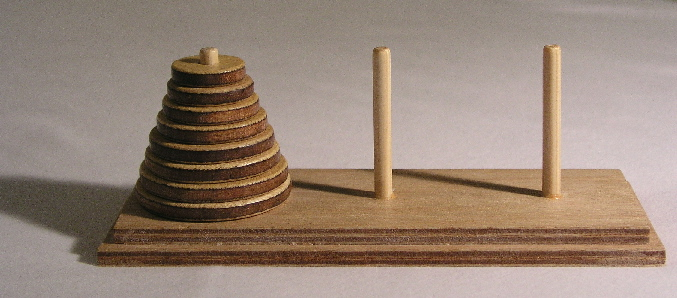
\includegraphics[width=1\linewidth]{Figures/Section_4/hanoi}
    \caption{Ein Modellset der Türme von Hanoi mit 8 Holzplatten \protect\cite{wikicommons}}
\end{figure}

\subsubsection{Theoretische Überlegungen}
Um das Problem zu lösen, wurde zunächst unabhängig vom Code über das Problem nachgedacht. Es wurde entschieden, das Problem physisch nachzubauen. Diese Methode half besonders dabei, das Problem zu verstehen und erste Überlegungen zur Abstraktion des Problems durchzuführen. Zunächst wurde versucht, durch zufälliges Ausprobieren eine Lösung zu finden. Dies funktionierte, allerdings wurden keine besonderen Muster gefunden, die bei einer allgemeinen Lösung des Problems helfen könnten.

Die ersten tatsächlichen Lösungsansätze waren sehr kompliziert, da noch kein globales Verständnis für das Problem vorhanden war. Zunächst wurde überlegt, wie das Problem abstrahiert werden kann. Ein erster Versuch, das Problem in einer algorithmischen Denkweise zu betrachten, erfolgte mit dem Aufstellen von mehreren Regeln. Wenn eine Platte auf mehrere Pole bewegt werden kann, wird diese auf den ersten verfügbaren Pol von links gesetzt. Wir beginnen am linkesten Pol und bewegen die Platten so lange auf einen anderen Pol, bis keine legalen Züge mehr möglich sind. Danach wird der nächste Pol von links betrachtet, bis keine legalen Züge mehr ausgeführt werden können, und so weiter.
Es wurde allerdings schnell beim Durchspielen dieses ersten Ansatzes am physischen Modell bemerkt, dass sich so schnell Endlosschleifen entwickeln.

In einem neuen Ansatz wurde das Problem in der reduziertesten Form betrachtet, mit insgesamt drei Holzplatten. Es zeigte sich, dass die größte Platte auf den rechtesten Pol zu setzen das erste "Teilziel" des Problems darstellt. Die anderen Platten werden durch Hilfsschritte geordnet und in der Mitte als Hilfspol zwischengelagert. Der Ansatz, auf Visualisierungen des Problems zurückzugreifen, half stark dabei, Muster in der Lösung zu erkennen.
Bei der Überlegung, wie man die Lösung nach dem funktionalen Paradigma umsetzen kann, fiel auf, dass Rekursion zwingend nötig sein wird. Falls mehr als 3 Holzplatten vorhanden sind, kann das Problem so lange weiter reduziert werden, bis nur noch drei Platten betrachtet werden. Von dort aus lässt sich das Problem rekursiv mit n-1 Platten lösen.

\subsubsection{Umsetzung}
% Abstraktion
Im nächsten Schritt wurde überlegt, wie das Problem auf eine virtuelle Welt abstrahiert werden kann. Die Holzplatten wurden hierbei als Integer dargestellt, um die Größen der Platten vergleichen zu können. Die Pole selbst wurden als Listen dargestellt, in denen jeweils das erste Element die oberste Holzplatte darstellt.
Ob ein Zug dem legalen Bewegungsset entspricht, wird anhand dessen bestimmt, ob das zu bewegende Element kleiner ist als das Element, auf dem dieses platziert wird. Elemente werden dann so lange bewegt, bis die "Win Condition" erreicht ist, in dem Fall, dass sich in den ersten beiden Listen keine Elemente mehr befinden.
Demnach gibt es eine Aufteilung der Verantwortungen, in denen zwei Funktionen die Gültigkeit und Zielbedingungen des aktuellen Zustandes prüfen, und eine Funktion, welche die tatsächlichen Züge durchführt und von den anderen beiden Hilfsfunktionen Gebrauch macht.

Da diese Funktion rekursiv laufen soll, muss sie alle nötigen Parameter entgegennehmen. Hierzu gehören der Startpol, Zielpol und ein Hilfspol, auf dem Platten zwischen platziert werden können. Zudem wird die Anzahl von Holzplatten benötigt, die sich in jedem rekursiven Schritt reduzieren soll.
Um das Endprodukt zu dokumentieren, wird zudem eine Liste von Lösungsschritten übergeben, die jeweils in einem Tupel den Startpol sowie den Endpol speichert. Hierbei muss aufgrund der Beschränkungen in der FP besonders darauf geachtet werden, wie die Lösungsschritte dokumentiert werden können. Diese können nicht etwa wie in einer prozeduralen Lösung nach jedem Schritt in der Konsole gedruckt werden, da FP keine Seiteneffekte zulässt.

% Tatsächliche Umsetzung
Die Umsetzung des Problems im funktionalen Paradigma erfolgte in Haskell. Zunächst wurden die Funktionsdefinitionen und Datenstrukturen geschrieben, und anschließend der Basisschritt und der rekursive Schritt.
Dabei fiel allerdings auf, dass die Umsetzung mit den einzelnen Polen als Listen von Integern nicht realistisch ist. Hierbei wurde in der Theorie zu sehr in herkömmliche prozedurale Denkstrukturen zurückgegriffen. Die Listen mit den Integern müssten demnach in jedem Schritt weiter verändert werden und haben somit eine Art Zustand, der nicht dem funktionalen Paradigma entspricht. Es wurde sich daher im Prozess der Implementierung entschieden, die Datenstrukturen wieder zu verwerfen und ausschließlich die Liste mit Lösungsschritten als Rückgabetyp zu geben. Da die Schrittfolge im Falle n=3 immer gleich ist und nur rekursiv wiederholt werden muss, müssen die Schritte zudem nicht gezwungenermaßen überprüft werden. Das Problem konnte letztendlich auf eine einzige Funktion mit nur einer Verantwortung reduziert werden. In einer späteren Reflexion der Lösung wurde entschlossen, dass dies die beste Lösung für eine funktionale Umsetzung ist.

\subsection{Zusammenhang mit Lerntypen}
Bei der Bearbeitung der Aufgabe konnten mehrere Beobachtungen gemacht werden, die sich direkt in Bezug auf die Erkenntnisse des Forschungsteils setzen lassen. Basierend auf den Ergebnissen des Fragebogens wurde erwartet, dass die mäßige Ausprägung der visuellen Dimension Vorteile für die Abstraktion und möglicherweise auch die Dekomposition mit sich bringt. Dabei ist letzteres abhängig von den gewählten Darstellungsmethoden während der Bearbeitung.
Tatsächlich erwies sich die Visualisierung des Problems durch einen physischen Nachbau als eine der hilfreichsten Strategien in der Lösungsfindung.
Auch das Aufteilen des Problems in Teilverantwortungen fiel leicht, jedoch ist dies unabhängig von den Vor- und Nachteilen des visuellen Lerntypen zu betrachten, da hierbei keine spezifischen visuellen Methoden eingesetzt wurden.

Hinsichtlich der aktiven/reflektiven Dimension wurden aufgrund eines leichten Hanges zum aktiven Typen mit Schwierigkeiten des reflektierten Arbeitens beim Debugging gerechnet. Tatsächlich ließ sich beobachten, dass eine sehr aktive Arbeitsweise verwendet wurde, bei der das schnelle Ausprobieren und Fehlschlagen im Vordergrund standen. Hierbei waren einige unterstützende Tools behilflich (siehe \nameref{sec:tools_prac}).
Im Nachhinein lässt sich sagen, dass diese Vorgehensweise im Kontext von FP nicht optimal war. Sie führte dazu, dass mehr Zeitaufwand für eine rekursive Lösung nötig war, als mit einer reflektierteren Arbeitsweise nötig gewesen wäre.

In der intuitiv/sensorischen Dimension wurden ebenfalls einige Hürden erwartet. Sensorische Typen haben eher Schwierigkeiten bei der Arbeit mit Abstraktion und Algorithmen als ihr Gegenpaar. Besonders in der FP lassen sich etablierte Methoden und Denkweisen nur schlecht anwenden, da sich das Paradigma stark von anderen Programmierstilen unterscheidet.
Im Kontext von FP bedeutet dies Schwierigkeiten bei der innovativen Entwicklung neuer Algorithmen, bei der Arbeit mit einem begrenzten Toolset, sowie Probleme beim rekursiven Denken.
Einer der am deutlichsten erkennbaren Schwierigkeiten im praktischen Teil war es, etablierte Methoden schlechter anwenden zu können, besonders um den Algorithmus allgemeiner und rekursiv zu gestalten. Es brauchte einen größeren Zeitaufwand, um sich auf die neue Denkweise umzustimmen.

In der sequenziell/globalen Dimension wurde ein recht ausgewogenes Verhältnis festgestellt, mit einer leichten Präferenz zum globalen Typ. Das Problem wurde in der theoretischen Lösungsfindung zunächst stark sequenziell betrachtet. Sobald ein ausreichendes globales Verständnis des Problems vorhanden war, fiel es einfach, die Funktionen letztendlich zu implementieren.
